\scanpage{126}
% archive sheet number: 125
% source lines 1--9
Voici quelques co\rlap{h}gitations dans ce sens, lorsque $C$ est muni d'un foncteur additif exact fidèle\deleted{F} $k$-linéaire $F:C\handwritten{\to}\rlap{(}M\mathrm{o}\rlap{\(\mathrm r\)}\mathrm{df}(k)$, et corresp\rlap{p}o\unsure{n|r} à ce titre à une algèbre profinie (ass un.) $U$, resp. une coalgèbre ass. unit. $A$, sur le corps $k$ (cf nº\handwritten{6}). On \deleted{voit que la donnée d} suppose donné une opération $\unsure{\otimes|\Omega}$, compatible avec $F$, i.e. un\deleted{e} hom. diagonal $U\handwritten{\to}U\overset{\handwritten{\scriptscriptstyle\wedge}}{\otimes}U$ i.e. une composition $A\otimes_kA\handwritten{\to}A$. On se propose de déterminer\inserted{\uline{to\unsure{$\mathbb{u}$|u}tes}\handwritten{\begin{tikzpicture}[x=.4cm,y=.4cm,baseline=-.2ex]\draw (0,-.45) .. controls (.06,-.08) and (.14,.17) .. (.42,.19)--(1.4,.18) .. controls (1.60,.18) and (1.75,.25) .. (1.72,.43);\end{tikzpicture}}} les données de symétrie $\handwritten{\psi}$ pour $\otimes$ (\uline{pas seulement} celles c\rlap{i}ompatibles avec le foncteur $F$ et la donnée de symmétrie ordinaire sur $\mathrm{Modf}(k)$ !) On trouve qu'\rlap{i}elles correspondent aux
\margin{\handwritten{[Dans le cas du nº 6, gr\uline{.dué}, on aura $\sigma=\pi^+\unsure{\ominus|\otimes}\pi^++\pi^+\otimes\pi^-+\pi^-\ominus\pi^+-\pi^-\ominus\pi^-$]}}
\[
\handwritten{\sigma\in}(U\overset{\handwritten{\scriptscriptstyle\wedge}}{\otimes}U)^{\handwritten{*}}
\tag*{\handwritten{(0)}}
\]
satisfaisant les conditions
\[
\left\{\begin{aligned}
&\handwritten{\sigma}'\handwritten{\sigma}=1\quad\text{(i.e. }\handwritten{\sigma}\text{ et }\handwritten{\sigma}'\text{ inverses l'un de l'autre: on aura aussi}\\
&\qquad\handwritten{\sigma\sigma}'=1,\quad\text{puisque }\handwritten{\sigma}\text{ es\handwritten{\begin{tikzpicture}[x=.4cm,y=.4cm,baseline=-.2ex]\draw (0,-.12) .. controls (.04,-.01) and (.13,.18) .. (.27,.31);\end{tikzpicture}}t supposé inversible)}\\
&\boxed{\handwritten{\sigma(\Delta}u)\handwritten{\sigma}^{-1}=\handwritten{(\Delta}u\handwritten{)}'\quad\text{pour tout }u\handwritten{\in}U}
\end{aligned}\right.
\tag*{\handwritten{(1)}}
\]
\margin{\handwritten{condition de symétrie ``tordue'' de l'application diagonale.}}
% source lines 14--18
en désignant par $x\handwritten{\mapsto}x'$ l'automorphisme de symétrie de $U\overset{\handwritten{\scriptscriptstyle\wedge}}{\otimes}U$. NB On ne dit pas que $\handwritten{\Delta}U$ est stable sous $x\handwritten{\mapsto}x'$, mais on considère $\handwritten{\Delta}$ et le symétrique $\handwritten{\Delta}'$ défini par $\handwritten{\Delta}'(u)=\handwritten{\Delta}(u)'$, qui définit la loi $\otimes$ \uline{opposée} de celle définie par $\handwritten{\Delta}$, et les relations entre $\handwritten{\sigma}$ et $\handwritten{\sigma}'$ sont symétriques et s'expriment\inserted{\handwritten{en disant}\handwritten{\begin{tikzpicture}[x=.4cm,y=.4cm,baseline=-.2ex]\draw (0,-.45) .. controls (.06,-.08) and (.14,.17) .. (.42,.19)--(1.8,.18) .. controls (2.00,.18) and (2.15,.25) .. (2.12,.43);\end{tikzpicture}}} que $\handwritten{\sigma}$ transforme $\handwritten{\Delta}$ en $\handwritten{\Delta}'$, $\handwritten{\sigma}'$ transforme $\handwritten{\Delta}'$ en $\handwritten{\Delta}$.

% source lines 19--22
Lorsqu'il y a une unité bilatère pour $\otimes$ et que $F$ est compatible avec celle-ci,\inserted{i.e. $A$ a\unsure{\rlap{s}d|\rlap{e}d}\rlap{t}met une unité bilatère,\handwritten{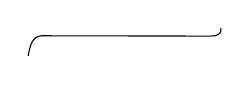
\begin{tikzpicture}[x=.4cm,y=.4cm,baseline=-.2ex]\draw (0,-.45) .. controls (.06,-.08) and (.14,.17) .. (.42,.19)--(5.8,.18) .. controls (6.00,.18) and (6.15,.25) .. (6.12,.43);\end{tikzpicture}}} alors la compatibilité de $\handwritten{\psi}$ à l'unité de $C$ s'exprime par les relations
\[
(\mathrm{id}_U\otimes\handwritten{\varepsilon}_U)(\handwritten{\sigma})=(\handwritten{\varepsilon}_U\otimes\mathrm{id}_U)(\handwritten{\sigma})=1,\quad\text{i.e.}\quad\handwritten{\varepsilon\in}1+U^{\handwritten{+}}\overset{\handwritten{\scriptscriptstyle\wedge}}{\otimes}U^{\handwritten{+}}.
\tag*{\handwritten{(2)}}
\]

% source lines 23--26 and bottom handwritten addition
Lorsqu'on a une donnée d'associativité \deleted{sur} $\handwritten{\phi}$ pour $\unsure{\otimes|\varpi}$, compatible avec $F$ et l'associativité ordinaire de $\otimes$ sur $\mathrm{Modf}(k)$, i.e. $A$ est associative, alors la compatibilité entre $\handwritten{\phi}$ et $\handwritten{\psi}$ s'exprime par une relation du style
\[
\deleted{\handwritten{\sigma}_1\handwritten{\sigma}_2\handwritten{\sigma}_3\handwritten{\sigma}'_1\handwritten{\sigma}'_2\handwritten{\sigma}'_3=1\handwritten{\unsure{\sigma}}}\quad\handwritten{(\mathrm{id}_U\widehat{\otimes}\Delta)(\sigma)\deleted{\sigma^{\unsure{23|13}}\sigma^{12}}=\deleted{1}\sigma^{12}\sigma^{13}}
\tag*{\handwritten{(3)}}
\]
\handwritten{où les $\sigma^{ij}$\inserted{\unsure{divers}\handwritten{\begin{tikzpicture}[x=.4cm,y=.4cm,baseline=-.2ex]\draw (0,-.45) .. controls (.06,-.08) and (.14,.17) .. (.42,.19)--(1.1,.18) .. controls (1.30,.18) and (1.45,.25) .. (1.42,.43);\end{tikzpicture}}} sont les 3 images de $\sigma'$ dans $U\ominus U\ominus U$ par $x\ominus y\mapsto x\ominus y\ominus1$ et les deux autres appl. analogues.}
